\smalltitle{سوال 1}
\begin{enumerate}
   \item در ابتدا به صورت پارامتری فرمول speedup را می‌نویسیم.
   در این مسئله
   $R$
   (که تعداد \lr{resourcse}هایی است که به هسته‌ی بزرگ دادیم)
   برابر است با
   $n^2$.
   پس
   $\operatorname{perf}(R) = n$
   است. همچنین تعداد هسته‌های کوچک برابر است با
   $64 - n^2$.
   همچنین مشخص است که
   $\operatorname{perf}(1) = 1$
   است.
   پس برای
   \lr{speedup}
   داریم:
   \begin{gather*}
        \frac{1}{0.3 \times \frac{1}{n} + 0.7 \times \frac{1}{64 - n^2}}
   \end{gather*}
   حال باید ببینیم که برای چه مقداری این عبارت بیشینه می‌شود.
   کافی است که برای حالت‌های مختلف
   $n$
   برای اعداد صحیح 1 تا 8 مقدار این عبارت را حساب کنیم و ببینیم که برای چه حالتی بیشینه می‌شود. به کمک
   \lr{desmos}
   این کار را انجام می‌دهیم:
    \begin{figure}[H]
        \centerline{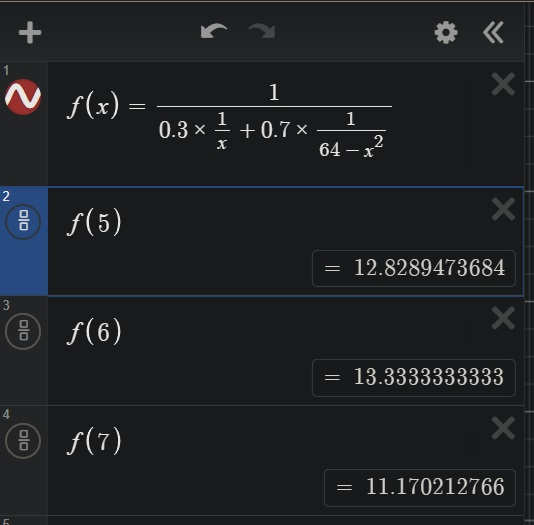
\includegraphics[scale=0.5]{pics/1-1.jpg}}
    \end{figure}
    پس برای حالت
    $n = 6$
    بیشترین سرعت را کسب می‌کنیم.
    \item در ابتدا قسمت سریال برنامه را در نظر می‌‌گیریم. در این قسمت کور‌های کوچک صرفا توان ایستا مصرف می‌کنند
    و کور بزرگ توان \lr{dynamic}. پس در این حالت $8 \times 6 + 0.35 \times (64 - 6^2) = 57.8W$ توان مصرفی ما است.
    در حالت موازی تمامی هسته‌ها در حال کار کردن هستند. پس توان ما برابر است با
    $6 + (64 - 6^2) = 34$.
    همان طور که در قسمت قبل نیز حساب کرده بودیم، زمان اجرای برنامه‌ی سری برابر
    $0.3 \times \frac{1}{6}$
    است و برنامه‌ی موازی برابر
    $0.7 \times \frac{1}{64 - 6^2}$
    است. پس در نهایت انرژی مصرفی برابر است با:
    \begin{gather*}
        0.3 \times \frac{1}{6} \times 57.8 + 0.7 \times \frac{1}{64 - 6^2} \times 34 = 3.74
    \end{gather*}
    \item \begin{enumerate}
        \item در این حالت داریم:
        \begin{gather*}
            \text{Speedup} = \frac{1}{0.3 \times \frac{1}{n} + 0.7 \times \frac{1}{n + 64 - n^2}} \stackrel{n = 6}{=} 14.167
        \end{gather*}
        در حالت قبلی داشتیم:
        \begin{gather*}
            \text{Speedup} = \frac{1}{0.3 \times \frac{1}{n} + 0.7 \times \frac{1}{64 - n^2}} \stackrel{n = 6}{=} 13.333
        \end{gather*}
        پس درصد بهبود برابر است با:
        \begin{gather*}
            \frac{14.167 - 13.333}{13.333} \times 100 \approx 6.25 \%
        \end{gather*}
        \item صرفا توان مصرفی در حالت موازی برابر است با:
        $6 \times 8 + (64 - 6^2) = 76$.
        پس انرژی مصرفی کلی برابر است با:
        \begin{gather*}
            0.3 \times \frac{1}{6} \times 57.8 + 0.7 \times \frac{1}{6 + 64 - 6^2} \times 76 \approx 4.45
        \end{gather*}
        \item اگر بخواهیم توان را نیز در نظر بگیریم مشخص است که این موضوع خیلی خوب نیست چرا که توان مصرفی به شدت
        افزایش یافت ولی سرعت به مقدار کمی افزایش یافت.
    \end{enumerate}
    \item در این حالت \lr{speedup} برابر است با:
    \begin{gather*}
        \frac{1}{S \times \frac{1}{5} + (1 - S) \times \frac{1}{64 - 5^2}}
    \end{gather*}
    که در این حالت $S$ برابر با مقدار کسر عملیات سریال است که در قسمت \lr{a} برابر \lr{0.3} بود.
    حال عبارت بالا را برابر
    \lr{13.333}
    قرار می‌دهیم که سرعت در قسمت
    \lr{a}
    بود. دوباره به کمک
    \lr{desmos}
    مقدار
    $S$
    را پیدا می‌کنیم.
    \begin{figure}[H]
        \centerline{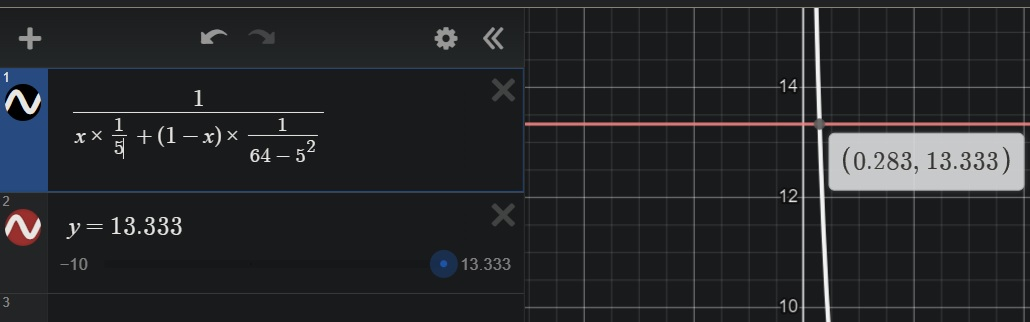
\includegraphics[scale=0.5]{pics/1-4.jpg}}
    \end{figure}
    پس اگر حدود
    $28.3\%$
    از پردازش ما سری باشد کافی است تا بتوانیم یکی از طول و عرض
    \lr{core}
    بزرگ کم کنیم.
    \item امکان پذیر نیست! چرا که در حال حالتی زمانی که قرار است سیستم پردازش موازی را انجام دهد، توان مصرفی
    هسته‌های کوچک ما برابر
    $64 - 6^2 = 28W$
    است. پس امکان ندارد که توان مصرفی همیشه زیر ۲۵ وات بماند.
\end{enumerate}








